\section{Demonstration}\label{sec:demo}

The demo setup consists of three machines and is illustrated in
figure~\ref{fig:demo-setup}. One machine is the game server. For this
purpose, we are using a four-core CPU, which gives us enough parallel
processing power to illustrate improvements over single threaded
implementations. Another machine plays back a trace of actual gameplay
in as many instances needed to emulate high loads on the server. The
client simulation machine is not a bottleneck, since simulating
clients requires very little calculation. The last machine is for
running the real game client, so the experimenter can see what is
going on on the server and play the actual game.

The demo setup also includes a wireless router and and a web-server
for sharing the game client with interested attendees. This setup
allows others to download the client and play the game during the demo
session.

\begin{figure}
\centering
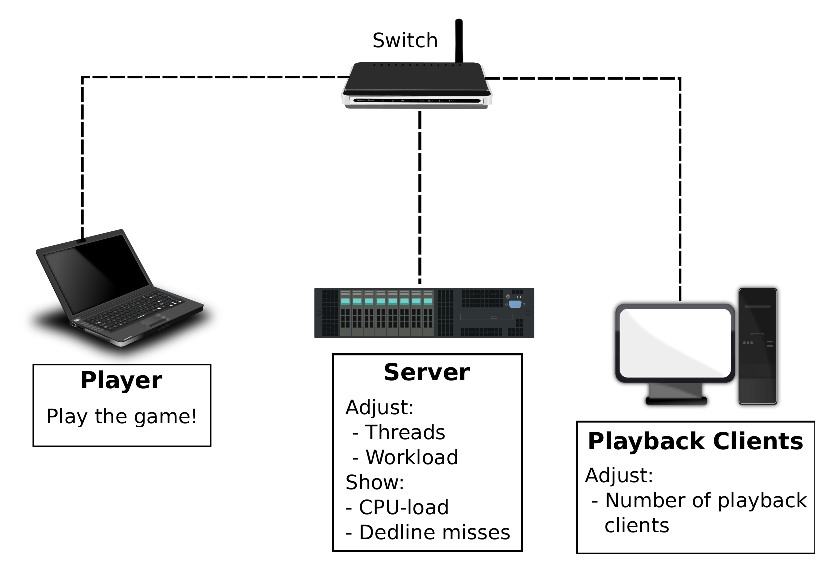
\psfig{file=FIG/demo-setup.eps,width=7cm}
\vspace{-1mm}
\caption{Setup of the demonstration}
\vspace{-2.5mm}
\label{fig:demo-setup}
\vspace{-2.5mm}
\end{figure}

For the purposes of this demonstration, the game server has been
updated with an interactive graphical user interface. Using this
interface, an experimenter can configure the conditions for the
experiment on the fly, while watching the results in real-time.

\begin{figure}
\centering
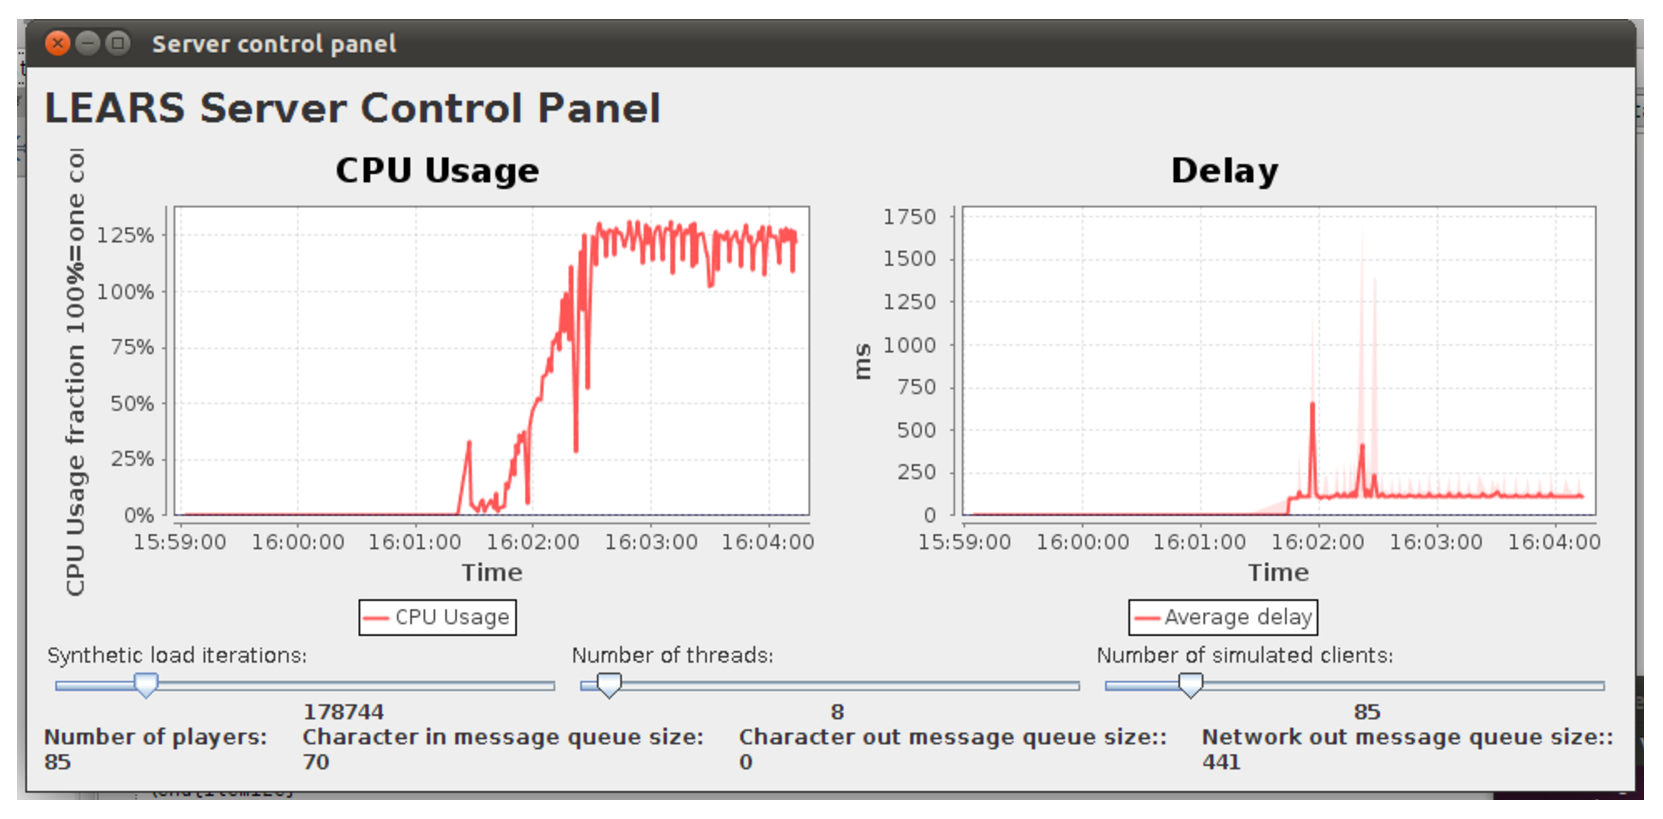
\psfig{file=FIG/gui.eps,width=9cm}
\vspace{-3mm}
\caption{Screenshot of the game server GUI}
\vspace{-2.5mm}
\label{fig:gui}
\vspace{-2.5mm}
\end{figure}

The GUI, shown in figure~\ref{fig:gui} has two plots, both updated
once every second. The left plot shows CPU usage vs. time. The right plot displays the interval between
updates. The system is designed to do an update every 100ms. Increases
above this level is considered deadline misses. The red line shows the
average value for the current measurement interval, the pink outline
shows the highest and lowest values. This is the main performance
metric for the server system, and any value above approximately 250ms
will severely deteriorate the QoE for players of the game.

Below the plots there are three sliders. One controls the number of
iterations for the synthetic load. The experimenter can adjust this to
change the intesnity of the load generated by each player. The next
slider sets the number of threads available to the thread pool. The
final slider instructs the playback client to start or stop playback
instances in order to reach the chosen number.

\section{Conclusion}
Using this setup it is possible to study, in real-time, how our
Lockless, Relaxed Atomicity State Parallel Game Server (LEARS) handles
different conditions, by varying the number of players, the number of threads and the synthetic load associated with each player.
The demo allows us to thoroughly investigate how the system reacts when the described parameters are changed.

Using this demonstration we can see clear indications that, if designed from the ground up with
parallelism in mind, game servers can scale well with the number of
cores on a unified memory multiprocessor system, even in the case
where all players must be aware of all other players and their
actions.
